\documentclass{beamer}
%\documentclass[handout]{beamer}

\usepackage{pgfpages} 

%\pgfpagesuselayout{4 on 1}[letterpaper,border shrink=5mm,landscape] 
%\pgfpagesuselayout{2 on 1}[letterpaper,border shrink=2mm]

\setbeameroption{show notes on second screen=left}
%\setbeameroption{show only notes}

\usetheme{default}

\mode<presentation> {
%  \usetheme{Warsaw}
  \usetheme{Frankfurt}
%  \usetheme{Boadilla}
%  \usetheme{Marburg}
}

\mode<handout>{\setbeamercolor{background canvas}{bg=black!5} %
    \pgfpagesuselayout{2 on 1}[letterpaper,border shrink=4mm] }

\title[CAC Intro] {An Introduction to MPI}
\author{Brock Palen\\ \texttt{brockp@umich.edu}}

\begin{document}
  \setbeamercovered{transparent}  
  \begin{frame}
    \titlepage
  \end{frame}

%table of contents
  \begin{frame}{Outline}
    \tableofcontents
  \end{frame}
  
\section{Overview}
 \subsection {What is MPI?}

\begin{frame}{MPI}
 \begin{block}{MPI}
   \begin{itemize}
     \item MPI - Message Passing Interface
       \note[item]{\url{http://en.wikipedia.org/wiki/Message\_Passing\_Interface}}
       \note[item]{MPI Standard: \url{http://www.mpi-forum.org/}}
     \item C/C++/F77/F90 Bindings
       \note[item]{\texttt{man MPI\_Send} for prototypes}
     \item Distributed Memory Programming
     \item Series of Functions
   \end{itemize}
 \end{block}
   \begin{block}{Assumptions}
     \begin{itemize}
       \item All examples work on \texttt{nyx-login.engin.umich.edu}
       \item Used with OpenMPI built with the PGI Compilers
     \end{itemize}
   \end{block}
\end{frame}

 \subsection{Alternatives}
  \begin{frame}{MPI's Flow}
   \begin{center}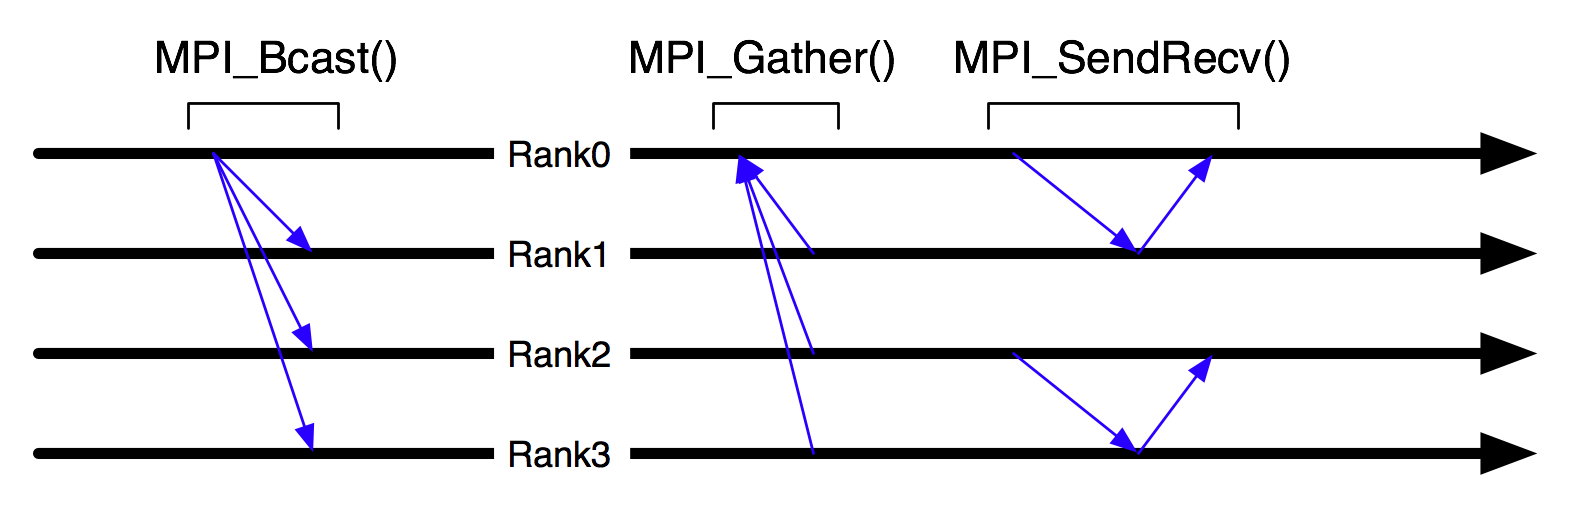
\includegraphics[height=1.5in]{mpi}\end{center}
    \note {MPI-All processes (normally one CPU per process but could be more) execute the same code. 
           These processes only know 'who they are' (their Rank). These ranks then have to explicitly 
           pass data.  This passing follows the form:
            \begin{enumerate}
              \item{Process 1 'Send to process 2'}
              \item{Process 2 'Recv from process 1'}
            \end{enumerate}
              \par Others options Collectives: \\ 
               \begin{itemize}
                \item {All process in a single Communicator,  'ALL DO THIS'}
               \end{itemize}
    } %note
  \end{frame}
  \begin{frame}{OpenMP}
   \begin{center}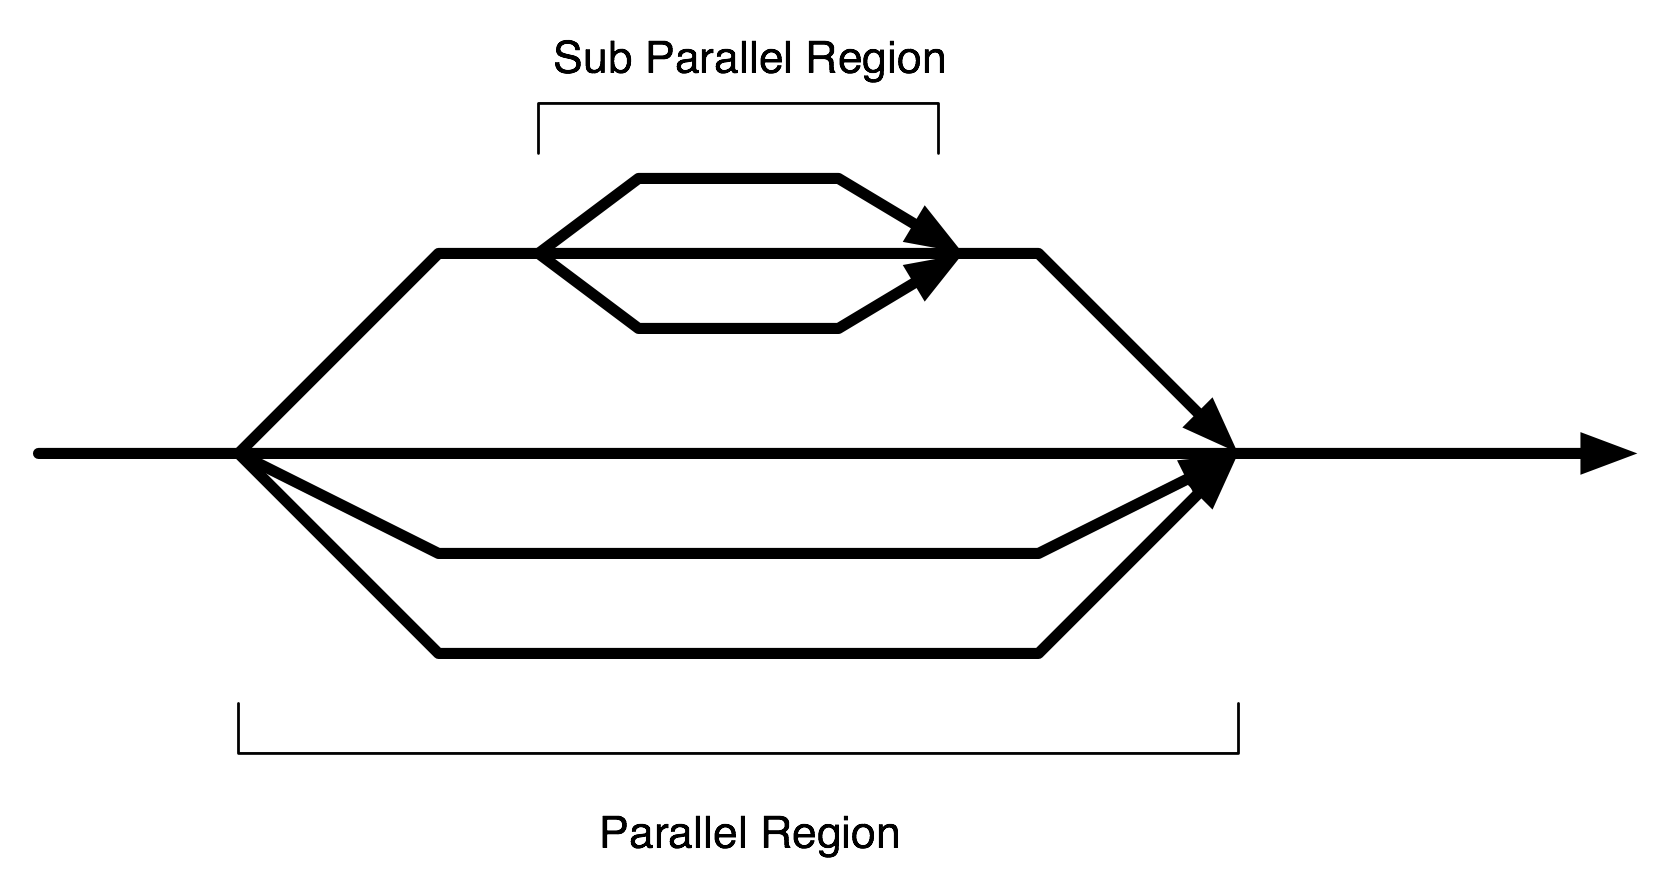
\includegraphics[height=2.5in]{openmp}\end{center}
   \note{OpenMP \url{http://www.openmpi.org} (Not to be confused with OpenMPI) is
         implemented in the compiler. Each compiler has its own issues with their 
         own implementation of OpenMP but most users should find no problems with the basics.
         \begin{itemize}
           \item Anything that uses \texttt{OMP\_NUM\_THREADS} uses OpenMP
           \item PGI Compilers: \texttt{pgf90 -mp openmp.f90}
           \item Intel Compilers: \texttt{ifort -openmp openmp.f90}
         \end{itemize}
   }
  \end{frame}
  \begin{frame}{Other Options}
    \begin{block}{Other Options}
     \begin{itemize}
      \item<1->HPF-High Performance Fortran -- Use OpenMP/MPI
       \note[item]{HPF, \url{http://hpff.rice.edu/}}
      \item<2->pthreads -- Use OpenMP
       \note[item]{pthreads, \url{http://en.wikipedia.org/wiki/POSIX\_Threads}}
      \item<3->PVM -- Dead, Not installed, Use MPI
       \note[item]{PVM,\url{http://www.csm.ornl.gov/pvm/}}
      \item<4->CoArray
       \note[item]{CoArray, \url{http://www.co-array.org/}}
      \item<4-> Shmem -- Use \texttt{MPI\_Get()} and \texttt{MPI\_Put()}
       \note[item]{Shmem, \url{http://www.sgi.com/products/software/mpt/}}
     \end{itemize}
    \end{block}
  \end{frame}

  \section{Code}
   \subsection{Mechanics}
   \begin{frame}{MPI Mechanics}
    \begin{block}{Parts of an MPI Message}
     \begin{itemize}
     \item<1->{ Address of data, called a buffer}
     \item<1->{ MPI Datatype}
     \item<1->{ Count, or number of MPI datatypes to message}
     \item<2->{ Tag, Used to separate messages from the same processor}
     \item<3->{ Communicator}
     \item<4->{ Rank of target}
     \end{itemize}
    \end{block}
    \note{
     MPI uses the buffer address, datatype and count to find how much raw data to send.
     For example, if MPI\_DOUBLE is 8 bytes, and count is 10, MPI 'knows' to send 80 bytes (10*8bytes) to the target process.  \\
     Note that \texttt{std::vector} is not a valid buffer for MPI! (or any STL class).  The STL does not make sure that all memory in continuous. This breaks MPI, remember all buffers must be well defined. 

  } %end note
   \end{frame}
  \subsection{Utility Functions}
  \begin{frame}[fragile]
  \frametitle{MPI\_Init() MPI\_Finallize()}
   \begin{columns}[T]
    \begin{column}{5cm}
     \begin{block}{C}
      \begin{semiverbatim}
MPI\_Init(int  *argc,
          char ***argv)

MPI\_Finalize()
      \end{semiverbatim}
     \end{block}
    \end{column}
    \begin{column}{5cm}
     \begin{block}{Fortran}
      \begin{semiverbatim}
INTEGER IERROR
MPI\_INIT(IERROR)

MPI\_FINALIZE(IERROR)
      \end{semiverbatim}
     \end{block}
    \end{column}
   \end{columns}
   \begin{itemize}
     \item<2-> MPI\_Init() and MPI\_Finalize() should only be called once
     \item<3-> No other MPI calls are valid outside these functions
   \end{itemize}
\end{frame}

\begin{frame}
 \frametitle{Communicators and Tags}
  \begin{block}{Communicators}
   \begin{itemize}
     \item<1->Specifies a group of processors that can communicate together
     \item<2->\texttt{MPI\_COMM\_WORLD}
     \item<2->Created at startup includes all processes started by the launcher
   \end{itemize}
  \end{block}
  \begin{block}{Tags}
    \begin{itemize}
     \item<3->Adds distinct meaning to a message
     \item<4->Very Useful
    \end{itemize}
  \end{block}
\note{
 \begin{itemize}
  \item \textbf{Communicators}
  \item There can be more than one communicator
  \item They can be duplicated \texttt{MPI\_Comm\_dup()}
  \item They can be created \texttt{MPI\_Comm\_create()}
  \item They can have physical meaning \texttt{MPI\_Cart\_create()}
 \end{itemize}
 \begin{itemize}
  \item \textbf{Tags}
  \item \texttt{MPI\_ANY\_TAG} 
  \item \texttt{Information on tag available in \texttt{MPI\_Status}}
 \end{itemize}
} %note

\end{frame}

\begin{frame}[fragile]
 \frametitle{MPI\_DATATYPE}
  \begin{columns}[T]
   \begin{column}{5cm}
    \begin{block}{C}
     \begin{itemize}
      \item \texttt{MPI\_CHAR char}
      \item \texttt{MPI\_INT int}
      \item \texttt{MPI\_FLOAT float}
      \item \texttt{MPI\_DOUBLE double}
      \item \texttt{MPI\_Pack() struct}
     \end{itemize}
    \end{block}
   \end{column}
   \begin{column}{5cm}
    \begin{block}{Fortran}
     \begin{itemize}
      \item \texttt{MPI\_CHARACTER CHARACTER}
      \item \texttt{MPI\_INTEGER INTEGER}
      \item \texttt{MPI\_REAL REAL}
      \item \texttt{MPI\_DOUBLE\_PRECISION DOUBLE}
      \item \texttt{MPI\_COMPLEX COMPLEX}
      \item \texttt{MPI\_DOUBLE\_COMPLEX DOUBLE\_COMPLEX}
     \end{itemize}
    \end{block}
   \end{column}
  \end{columns}
 \note{
 \begin{itemize}
  \item Unsigned and shorts also available
  \item Fortran can use \texttt{MPI\_REAL8 MPI\_INTEGER2} etc.
  \item C Structs must be 'packed' with \texttt{MPI\_Pack()}
  \item \url{http://www.lam-mpi.org/tutorials/one-step/datatypes.php}
 \end{itemize}
} %note
\end{frame}

\subsection{Point to Point}
\begin{frame}[fragile]
 \frametitle{MPI\_Send()}
   \begin{columns}[T]
    \begin{column}{5cm}
     \begin{block}{C}
      \begin{semiverbatim}
MPI\_Send( void  *buf,
           int count,
  MPI\_Datatype  type,
           int  dest,
           int   tag,
      MPI\_Comm   comm)
      \end{semiverbatim}
     \end{block}
    \end{column}
    \begin{column}{5cm}
     \begin{block}{Fortran}
      \begin{semiverbatim}
MPI\_SEND( <type>   BUF,
      INTEGER    COUNT,
 MPI\_Datatype     TYPE,
      INTEGER     DEST,
      INTEGER      TAG,
     MPI\_Comm     COMM,
      INTEGER    IERROR)
      \end{semiverbatim}
     \end{block}
    \end{column}
   \end{columns}
\note{
These are called 'blocking' sends. Note that MPI does not require that \texttt{MPI\_Send()} block, just that it not return until \texttt{buf} is safe to use again. This can cause deadlocks to appear in code when scaled up. See the example included with this.
} %note
\end{frame}
\begin{frame}[fragile]
 \frametitle{MPI\_Recv()}
   \begin{columns}[T]
    \begin{column}{5cm}
     \begin{block}{C}
      \begin{semiverbatim}
MPI\_Recv( void   *buf,
           int  count,
  MPI\_Datatype   type,
           int source,
           int    tag,
      MPI\_Comm   comm,
    MPI\_Status  *status)
      \end{semiverbatim}
     \end{block}
    \end{column}
    \begin{column}{5cm}
     \begin{block}{Fortran}
      \begin{semiverbatim}
MPI\_RECV( <type>    BUF,
      INTEGER     COUNT,
 MPI\_Datatype      TYPE,
      INTEGER    SOURCE,
      INTEGER       TAG,
     MPI\_Comm      COMM,
      INTEGER    STATUS,
      INTEGER     IERROR)
      \end{semiverbatim}
     \end{block}
    \end{column}
   \end{columns}
\note{
In Fortran STATUS must be: \texttt{integer status(MPI\_STATUS\_SIZE)}
The same issues apply here as MPI send. For every \texttt{MPI\_Send()} there must be a \texttt{MPI\_Recv()}. Most codes will put most of their communication time waiting for Recv's to actually get their data. If there is no Send, Recv will wait forever.  See \texttt{MPI\_Irecv()} for non-blocking.
} %note
\end{frame}

\begin{frame}{First MPI Program}
\begin{block}{helloworld}
 \begin{enumerate}
  \item<1->\texttt{cp \~{}brockp/mpi-cac.tar.gz \~{}}
  \item<1->\texttt{tar -xzvf mpi-cac.tar.gz}
  \item<1->\texttt{cd mpi-cac}
  \item<2-> C: \texttt{mpicc -o chello helloworld.c}
  \item<2-> F90: \texttt{mpif90 -o fhello helloworld.f90}
  \item<3-> mpirun -np 4 fhello
 \end{enumerate}
\end{block}
 \note{
  \texttt{mpi-cac.tar.gz} includes a \texttt{Makefile} all examples can be built by running \texttt{make} or built one at a time, \texttt{make chello} will build the \texttt{helloworld.c} example.  While \texttt{make fapps} will build all Fortran examples.  See \texttt{README} included for information.
 } %note
\end{frame}

\begin{frame}{Deadlocks}
 \begin{block}{Deadlock}
   \begin{itemize}
    \item Every \texttt{MPI\_Send()} must have a matching \texttt{MPI\_Recv()}
    \item A call that does not have a matching Send or Recv is deadlocked
    \item Calls do not return unless \texttt{buffer} is safe to reuse, \alert{not} that it was received
    \item Some MPI libraries will let deadlocked code run until messages reach a given size
   \end{itemize}
 \end{block}
 \begin{block}{cdeadlock}
  \begin{itemize}
   \item <2->\texttt{make cdeadlock no-cdeadlock}
   \item <2->\texttt{mpirun -np 4 cdeadlock}
   \item <2->\texttt{mpirun -np 4 no-cdeadlock}
  \end{itemize}
 \end{block}
 \note{
    This example will demonstrate the effects of deadlock, and eager messages. \\
    cdeadlock and no-cdeadlock is the same code, the change is in the size of \texttt{buffer} when buffer falls below some value eager messaging takes place. In this case the MPI library says the message is small enough, lets allocate memory copy the buffer to it and return right away, so the buffer is now safe to reuse allowing the code to continue.  In the cdeadlock/fdeadlock case these buffers are to large and MPI
 will not copy the code will block at \texttt{MPI\_Send()}  for forever.
} %note
\end{frame}

\begin{frame}{Deadlock Example}
   \begin{center}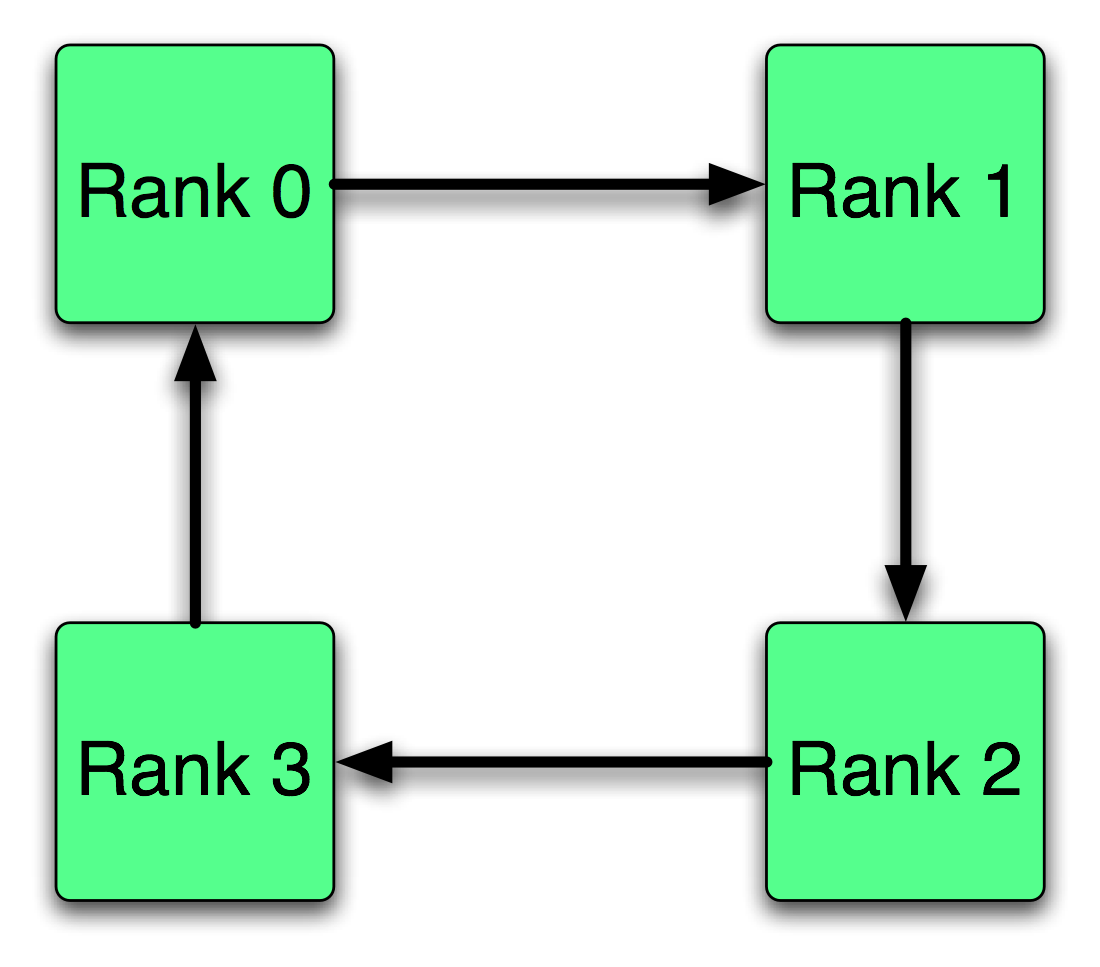
\includegraphics[height=3.0in]{deadlock}\end{center}
   \note{
    \begin{itemize}
      \item Each process does a \texttt{MPI\_Send()} to rank+1
      \item Each process then calls \texttt{MPI\_Recv()} from rank-1
      \item \texttt{make cdeadlock} or \texttt{make fdeadlock}
      \item \texttt{mpirun -np 4 cdeadlock}
      \item \texttt{make no-cdeadlock} or \texttt{make no-fdeadlock}
    \end{itemize}
} %notes
\end{frame} 
\begin{frame}{Non-Blocking Functions}
\begin{block}{MPI\_Isend() MPI\_Irecv()}
  \begin{itemize}
   \item Example \texttt{non-blocking.c/non-blocking.f90}
   \item Can mix blocking with non blocking
   \item \texttt{MPI\_Isend() -> MPI\_Recv()}
   \item Uses \texttt{MPI\_Request} opbjects
   \item \texttt{MPI\_Test() MPI\_Wait()} etc.
  \end{itemize}
\end{block}
\note{
   \texttt{MPI\_Wait()} will block waiting for the send or recv to complete.  \texttt{MPI\_Test()} returns if a message has completed. You can \alert{not} touch the buffer once it is used in a request. Once the request has been completed by checking with \texttt{MPI\_Wait()} or \texttt{MPI\_Test()} the buffer may be reused.
\begin{itemize}
  \item \texttt{MPI\_Testany() MPI\_Waitany()}
  \item These calls have overhead the blocking calls don't
  \item The overhead of complicated programming
  \item Overhead for more complicated communication may outweigh benefits
\end{itemize}
} %note
\end{frame}

\subsection{Collectives}
\begin{frame}{Collectives}
\begin{block}{Collectives}
 Collectives work on a entire communicator of processes
 \begin{itemize}
  \item <2->\texttt{MPI\_Barrier()} Blocks till all ranks reach a single point
  \item <2->\texttt{MPI\_Bcast()} Send data from one rank to all others
  \item <3->\texttt{MPI\_Reduce()} Do a operation on data on all processors and store result on a single rank
  \item <4->\texttt{MPI\_Scatter()} Scatter data from one CPU to many
  \item <5->\texttt{MPI\_Gather()} Gather data and put on a single rank
 \end{itemize}
\end{block}
\note{
  All these collective functions have a 'All' version (\texttt{MPI\_Allreduce()}) which has the results end on all cpus.  For example \texttt{MPI\_Allreduce()} puts the results of the reducing operation on all ranks not just a single rank.\\ Other functions to look at:
\begin{itemize}
 \item \texttt{MPI\_Allreduce()}
 \item \texttt{MPI\_Allscatter()}
 \item \texttt{MPI\_Allgather()}
 \item \texttt{MPI\_Alltoall()}
\end{itemize}
} %note 
\end{frame}

\begin{frame}[fragile]
\frametitle{MPI\_Bcast()}
   \begin{columns}[T]
    \begin{column}{5cm}
     \begin{block}{C}
      \begin{semiverbatim}
MPI\_Bcast(void   *buf,
           int  count,
  MPI\_Datatype   type,
           int   root,
      MPI\_Comm   comm)
      \end{semiverbatim}
     \end{block}
    \end{column}
    \begin{column}{5cm}
     \begin{block}{Fortran}
      \begin{semiverbatim}
MPI\_BCAST( <type>    BUF,
         INTEGER   COUNT,
    MPI\_Datatype    TYPE,
         INTEGER    ROOT,
        MPI\_Comm    COMM,
         INTEGER  IERROR)
      \end{semiverbatim}
     \end{block}
    \end{column}
   \end{columns}
\note{
\texttt{root} is the rank you wish to broadcast data from. Root must be specified and the same on all ranks in \texttt{comm}. \\ 
If you need every rank to broadcast its data to every other process (A very inefficient operation) the function is \texttt{MPI\_Alltoall()} 
} %note
\end{frame}
\begin{frame}[fragile]
\frametitle{MPI\_Reduce()}
   \begin{columns}[T]
    \begin{column}{5cm}
     \begin{block}{C}
      \begin{semiverbatim}
MPI\_Reduce(void *sendbuf,
           void *recvbuf,
            int    count,
   MPI\_Datatype     type,
         MPI\_Op       op,
            int     root,
       MPI\_Comm     comm)
      \end{semiverbatim}
     \end{block}
    \end{column}
    \begin{column}{5cm}
     \begin{block}{Fortran}
      \begin{semiverbatim}
MPI\_REDUCE(<type> SENDBUF,
           <type> RECVBUF,
          INTEGER  COUNT,
     MPI\_Datatype   TYPE,
          MPI\_Opt     OP,
          INTEGER   ROOT,
         MPI\_Comm   COMM,
          INTEGER IERROR)
      \end{semiverbatim}
     \end{block}
    \end{column}
   \end{columns}
\note{
\begin{itemize}
  \item \texttt{root} is the rank that the results of \texttt{op} should go to
  \item \texttt{*recvbuf} does need to be defined on all ranks
\end{itemize}
}%
\end{frame}
\begin{frame}{MPI Operations}
  \begin{block}{MPI\_Op}
   \begin{columns}[T]
   \begin{column}{5cm}
   \begin{itemize}
    \item MPI\_MAX
    \item MPI\_MIN
    \item MPI\_PROD
    \item MPI\_SUM
    \item MPI\_LAND
    \item MPI\_LOR
    \item MPI\_LXOR
   \end{itemize}
   \end{column}
   \begin{column}{5cm}
    \begin{itemize}
    \item MPI\_BAND
    \item MPI\_BOR
    \item MPI\_BXOR
    \item MPI\_MAXLOC
    \item MPI\_MINLOC
    \end{itemize}
   \end{column}
  \end{columns}
  \end{block}
  \note{
   \begin{itemize}
    \item LAND, LOR, LXOR: Logical AND, Logical OR, Logical XOR.
    \item BAND, BOR, BXOR: Bitwise AND, Bitwise OR, Bitwise XOR.
   \end{itemize}
   
   Use \texttt{MPI\_Reduce\_scatter()} to reduce the buffers with \texttt{MPI\_Op} and then scatter (to be covered) the results to all ranks. Rather than using two calls.
  }%note
\end{frame}

\begin{frame}{fpi.f90}

\begin{block}{Calculate pi}
\[
\int^1_0 \frac{4}{1+x^2}\,dx = \pi
\]
\begin{enumerate}
 \item <2->Break into \texttt{n} rectangles
 \item <3->Have each rank work on a subset of these
 \item <4->Find a global sum from partial sums
\end{enumerate}
\end{block}
\begin{block}{fpi.f90}
 \texttt{make fpi} \\
 \texttt{mpirun -np 4 fpi}
\end{block}
\note{
 \textbf{Details}
\begin{itemize}
 \item Rank 0 asks the number of intervals from the user and uses \texttt{MPI\_Bcast()} to other ranks
 \item Ranks work on a subset of the intervals. Ranks step by n+nproc intervals each iteration
 \item All ranks use \texttt{MPI\_Reduce()} with \texttt{MPI\_SUM} to find a global total
 \item Rank 0 then normalizes and displays output
\end{itemize}
}
\end{frame}

\begin{frame}{MPI\_Scatter() MPI\_Gather()}
  \begin{itemize}
   \item <1->\texttt{MPI\_Scatter()}
   \item <2->\texttt{MPI\_Gather()} is the reverse
  \end{itemize} 
   \begin{center}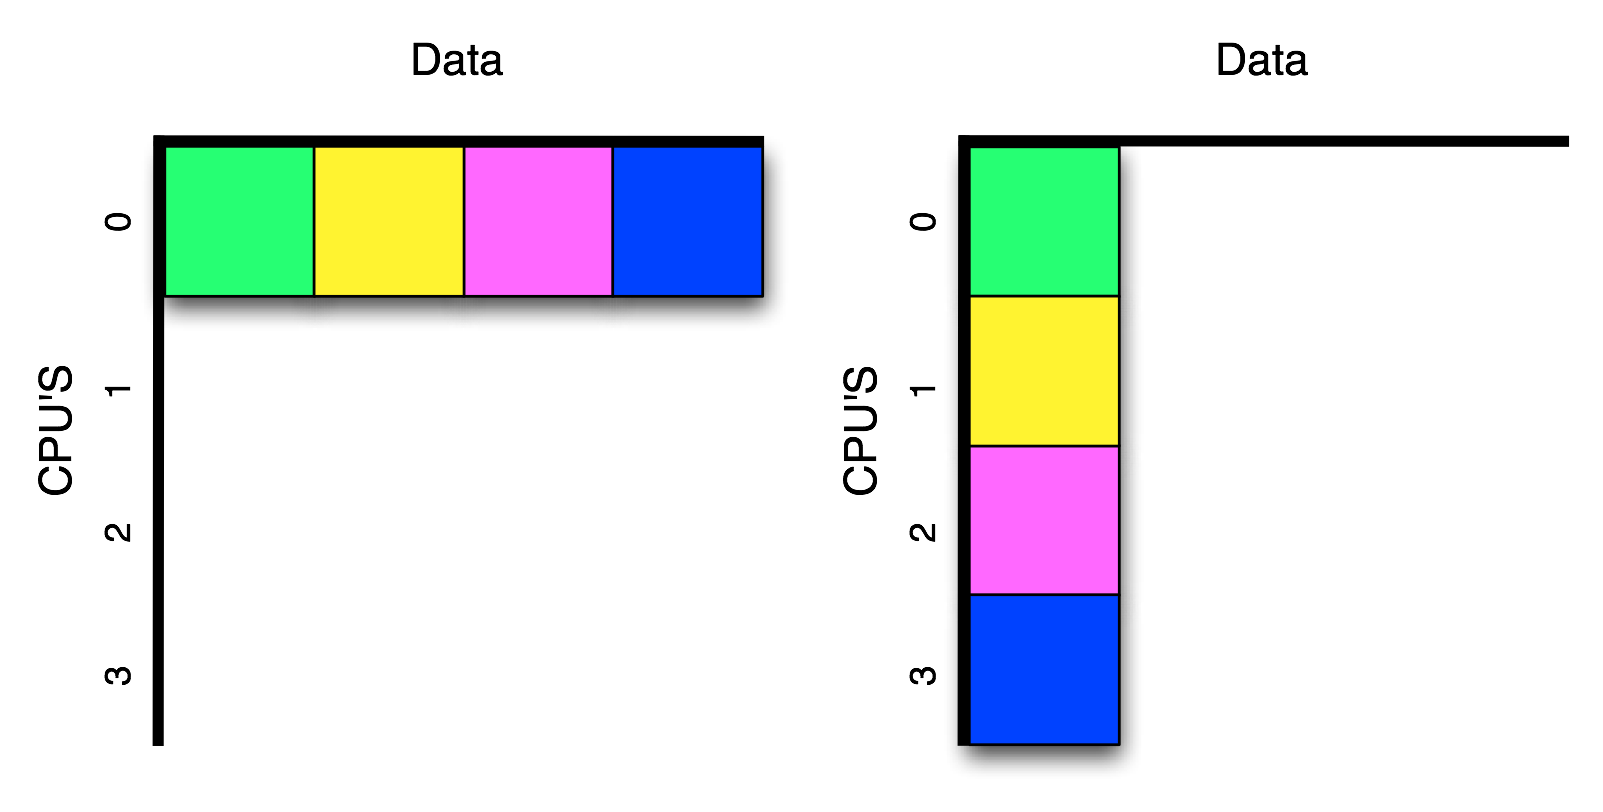
\includegraphics[height=2.2in]{scatter}\end{center}
 \note{
  \texttt{MPI\_Scatter()} takes data on a single rank breaks it evenly among all the ranks leaving each rank with a small portion of the entire set of data in its output buffer.  \\
   It is commonly useful to combine \texttt{MPI\_Scatter()} with \texttt{MPI\_Reduce()}. MPI defines a function that does this for you: \texttt{MPI\_Reduce\_scatter()}. This is different than \texttt{MPI\_Allreduce()} because the reduced data is not cloned across all ranks but broken in pieces across all ranks.\\
Because sometimes each rank is not to get the same amount of data from a Scatter or Gather MPI defines: \texttt{MPI\_Scatterv(), MPI\_Gatherv()} and \texttt{MPI\_Allgatherv()}. These calls take an extra \texttt{displs} option that describes how much data each rank should receive. See the \texttt{man} pages for these calls.
 } %note
\end{frame}

\begin{frame}{MPI\_Allgather()}
   \begin{center}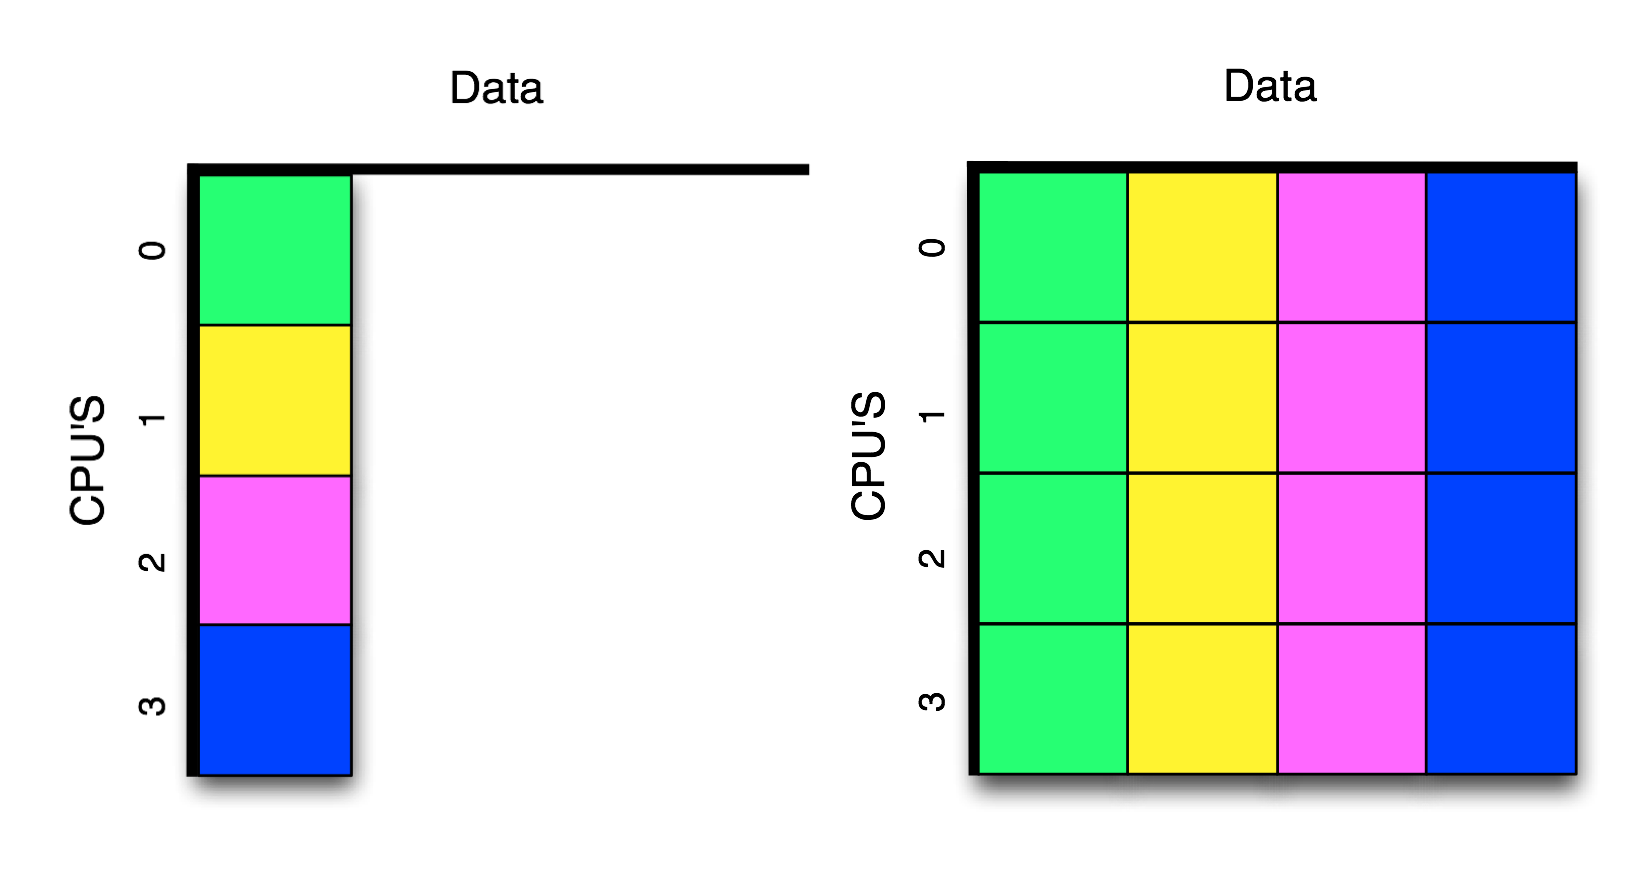
\includegraphics[height=2.2in]{allgather}\end{center}
 \note{
\texttt{MPI\_Allgather()} collects distributed data like \texttt{MPI\_Gather()} but then distributes this data to all ranks in the communicator. This behavior could be simulated with \texttt{MPI\_Gather()} followed by \texttt{MPI\_Bcast()}. As always use the single collective not the two latter together. 
} %note
\end{frame}

\begin{frame}{Warnings with Collectives}
 \begin{block}{Avoid}
  \begin{itemize}
   \item \texttt{MPI\_Barrier()}
   \item \texttt{MPI\_Alltoall()} 
   \item \texttt{MPI\_Allreduce()}
   \item \texttt{MPI\_Allreduce()}
   \item \texttt{MPI\_All*()}
  \end{itemize}
 \end{block}
\note{
While I point out to avoid these calls its because of the communication complexity. For example \texttt{MPI\_Alltoall()} in its worse form is: \[O(n^{2}-n)\] You should not try to mimic its behavior by mixing other calls.  What should be done is find a algorithm that does not require such a exchange. If this is not the case \textbf{do} make sure to use \texttt{MPI\_Alltoall()}.  This applies to all other mentioned calls. \\

\texttt{MPI\_Barrier()} gets abused. Its use normally is not needed.  Because most other MPI calls block such synchronization is implied.  Using a barrier is really only good for timing with \texttt{MPI\_Wtime()}
} %note
\end{frame}

\section{Summary}
\subsection{Advanced MPI}
\begin{frame}{Advanced Calls}
 \begin{block}{Topology}
 \begin{itemize}
  \item\texttt{MPI\_Cart\_create()} creates a communicator with Cartesian topology.
 \end{itemize}
 \end{block}
 \begin{block}{Timing}
  \begin{itemize}
   \item \texttt{MPI\_Wtime()} Time in seconds from arbitrary time in the past.
   \item \texttt{MPI\_Wtick()} Returns resolution of \texttt{MPI\_Wtime()}
  \end{itemize}
 \end{block}
\end{frame}

\subsection{Documentation}
\begin{frame}{Documentation}
\begin{block}{Documentation}
 \begin{itemize}
  \item Use the \texttt{man} pages on the CAC systems.
  \item Google/Yahoo Etc.
  \item CoE EECS 587
  \item "Using MPI" -- Gropp, Lusk, and Skjellum  
  \item "Parallel programming in C with MPI and OpenMP" -- Quinn
  \item "Parallel scientific computing in C++ and MPI" -- Karniadakis, Kirby
 \end{itemize}
\end{block}
 \note{
 Many books are available in Mirlyn:\\
 \begin{itemize}
  \item "Parallel programming in C with MPI and OpenMP" QA 76.73 .C15 Q551 2004
  \item "Parallel scientific computing in C++ and MPI" QA 76.58 .K371 2003
 \end{itemize}
} %

\end{frame}

\subsection{Contact}
\begin{frame}{Contact Us}
 \begin{block}{Support}
  \begin{itemize}
   \item \url{http://cac.engin.umich.edu}
   \item cac-support@umich.edu
  \end{itemize}
 \end{block}
\end{frame}
\end{document}
